%%%%%%%%%%%%%%%%%%%%%%%%%%%%%%%%%%%%%%%%%
% Seismica Submission: Software Report
% Compile:  pdflatex node_toolbox_seismica; bibtex node_toolbox_seismica;
%           pdflatex node_toolbox_seismica; pdflatex node_toolbox_seismica
% Figures:  python make_figures.py   (writes figures/)
%%%%%%%%%%%%%%%%%%%%%%%%%%%%%%%%%%%%%%%%%

\documentclass[report]{seismica}

\title{Data management of SmartSolo node-type geophones using open-source Python}
\shorttitle{Open-source tools for SmartSolo node data}

\reporttype{Software Report}

%-----------------------------------------
%% AUTHORS  (TODO: check ORCID, affiliation, add co-authors)
\author[1]{Tobias St{\aa}l
\orcid{0000-0000-0000-0000}
\thanks{Corresponding author: tobias.staal@utas.edu.au}
}
\affil[1]{University of Tasmania, Hobart, Tasmania, Australia}

\credit{Conceptualization}{Tobias St{\aa}l}
\credit{Methodology}{Tobias St{\aa}l}
\credit{Software}{Tobias St{\aa}l}
\credit{Validation}{Tobias St{\aa}l}
\credit{Investigation}{Tobias St{\aa}l}
\credit{Data Curation}{Tobias St{\aa}l}
\credit{Visualization}{Tobias St{\aa}l}
\credit{Writing - Original draft}{Tobias St{\aa}l}

\begin{document}

\makeseistitle{
\begin{summary}{Abstract}
Autonomous three-component nodes such as the SmartSolo IGU-16HR are now common in passive seismology, but their data arrive in an undocumented binary format and with state-of-health logs that are usually read through vendor software on Windows. We present node\_toolbox, an open-source Python package that reads every file a SmartSolo node writes. It parses the logs into a time-indexed pandas table, derives one deployment per power-up from the first stable GPS position, and selects deployments by radius, polygon and time. It reads the raw DLD data files directly, without vendor software, and cuts the selected windows into MiniSEED or SEG-Y with StationXML metadata, polarity correction and instrument response. It also analyses the geophone pulse test and the compass and tilt records. While documenting the DLD format we found that the time text in each data block is 2~s late until the GPS receiver has learned the leap seconds; the GPS time of week in the same block is not affected, and the reader uses it. We verify the package with unit tests, two Antarctic nodes and a six-node vehicle braking test. The repository contains the code, tests, example data and tutorial notebooks.
\end{summary}
\begin{summary}{Non-technical summary}
Small, self-contained seismic sensors called nodes are planted in large numbers to record ground vibrations from earthquakes, ice and traffic. Each node stores its recordings and a diary of its health: temperature, battery, GPS position and tilt. For one widely used brand, SmartSolo, these files are normally opened with the manufacturer's Windows program. We wrote free Python software that reads all of these files directly. It works out where and when each sensor was recording and cuts out the data for chosen places and times. It saves them in the standard formats seismologists share, together with a description of each sensor. It also checks whether the sensors worked properly. We found and corrected a hidden 2-second timing error in how the files label time. We tested the software on sensors left for two weeks on the Antarctic ice and on six sensors beside a road in Hobart, Australia, where a four-wheel-drive car braked repeatedly.
\end{summary}
}

%-----------------------------------------
\section{Introduction}

Autonomous geophone nodes, which combine a 5~Hz three-component sensor, a 24-bit digitizer, a GNSS receiver, a battery and storage in one sealed unit, have made dense passive arrays practical \citep{karplus_preface_2018,ringler_nodes_2018}. Their ease of deployment is especially valuable where logistics are constrained, such as on the Antarctic ice sheet, where every kilogram flown and every minute spent at a site counts. The SmartSolo IGU-16HR 3C (DTCC) is among the most widely used of these instruments \citep{zeckra_smartsolo_2022}.

Deploying many nodes, however, shifts the work to data management. A SmartSolo node stores its raw samples in an undocumented binary format (\code{.DLD}), and writes its state of health to a text log (\code{DigiSolo.LOG}) whose content changes between firmware versions. The usual workflow is to harvest and export the data with the vendor's Windows software (SoloLite). The positions, orientation and quality-control information are then transferred by hand into station metadata. Several pitfalls in this chain are known. All IGU-16HR channels have negative polarity relative to the FDSN convention. A missing leap-second configuration file leads to an 18-s timing error at export. The programmed preamplifier gain must be removed consistently \citep{auspass_nodes,auspass_data}. Field crews also need to know when a node was moved, tilted or tested while being handled, which is recorded in the logs but rarely used.

Here we describe node\_toolbox \citep{node_toolbox}, a pure-Python package for SmartSolo node data built on ObsPy \citep{beyreuther_obspy_2010,krischer_obspy_2015}, pandas \citep{mckinney_pandas_2010}, NumPy \citep{harris_numpy_2020}, SciPy \citep{virtanen_scipy_2020}, GeoPandas \citep{jordahl_geopandas_2020} and Matplotlib \citep{hunter_matplotlib_2007}. The package (i) parses state-of-health logs from all firmware versions we have seen into one time-indexed table, (ii) derives deployments and selects them in space and time, (iii) reads the raw \code{.DLD} files directly, (iv) writes MiniSEED, SEG-Y \citep{seg_segy_2017} and StationXML \citep{fdsn_stationxml} with polarity, gain and response handled, and (v) provides sensor quality control from the pulse test, boot-time geophone tests, compass and tilt. We document the \code{.DLD} format, including a timing behaviour that affects any reader of these files. We then verify the package on two Antarctic nodes and a six-node braking test.

%-----------------------------------------
\section{Instrument and files}

Each node writes the files listed in Table~\ref{tab:files}. Harvesting with SoloLite copies them into a folder named after the serial number and harvest time, but node\_toolbox does not depend on that layout. Serial numbers are taken from file contents where possible, otherwise from paths. The examples in this paper come from nodes with firmware V1.0.5.6kp, V1.0.8.1be, V1.1.2.0be and V1.1.4.2be recording at 250, 500 and 1000 samples per second (sps).

\begin{table*}[ht!]
\seismicatablestyle
\begin{tabular}{m{3.6cm} m{6.4cm} m{6.2cm}}
File & Content & Module \\
\hline
\code{DigiSolo.LOG} & state-of-health log: boots, GPS, temperature, battery, memory, compass/tilt, boot-time geophone test & \code{smartsolo\_log}, \code{smartsolo\_locate}, \code{smartsolo\_orientation} \\
\code{seisNNN\{X,Y,Z\}.DLD} & raw samples, one file per component and power-up, with GPS time and position tags & \code{smartsolo\_dld} \\
\code{PULSE\_\{X,Y,Z\}.WAV} & geophone pulse test of the latest power-up & \code{smartsolo\_node} \\
\code{sct\_par.xml}, \code{SCT\_INT.XML} & acquisition script with test limits & \code{smartsolo\_node} \\
\code{device.ini} & serial number and firmware (not on all nodes) & \code{smartsolo\_node} \\
SoloLite MiniSEED/SEG-Y & optional exported waveforms & \code{smartsolo\_waveforms} \\
\end{tabular}
\caption{Files written by a SmartSolo IGU-16HR node and the node\_toolbox module that reads them.}
\label{tab:files}
\end{table*}

%-----------------------------------------
\section{Software design}

node\_toolbox consists of six modules (Fig.~\ref{fig:workflow}; about 3000 lines of Python). They exchange plain data structures rather than custom classes. Logs become a pandas DataFrame with a UTC time index. Deployments become a GeoDataFrame, waveforms an ObsPy \code{Stream} and metadata an ObsPy \code{Inventory}. A user can therefore stop at any stage and continue with standard tools, for example to plot the temperature of every node with one line of pandas. All times are UTC. Every function that guesses (a position, a time convention, a polarity) records what it did in a table column, so that the choice can be audited.

\begin{figure*}[ht!]
\centering
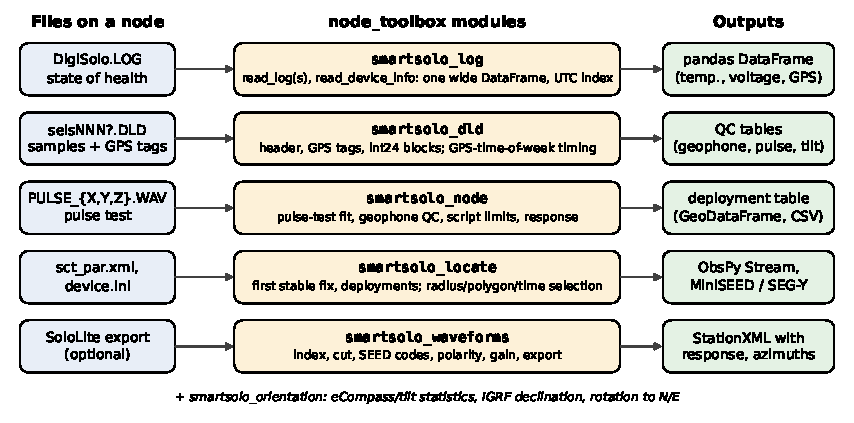
\includegraphics[width=\textwidth]{figures/fig01_workflow.pdf}
\caption{Structure of node\_toolbox. Files written by a node (left) are read by the modules (centre), which return pandas, GeoPandas and ObsPy objects and standard files (right).}
\label{fig:workflow}
\end{figure*}

\subsection{State-of-health logs}

\code{DigiSolo.LOG} is an INI-like text file of numbered sections (e.g.\ \code{[DeviceInfo00001]}, \code{[GPS00042]}). Its first line lists the number of DeviceInfo, GPS, Temperature, Memory, Battery, Error and Notify records. \code{smartsolo\_log.read\_log} turns each section into one row of a single wide DataFrame, one column per key in snake case, indexed by the record's UTC time. The record type, record number, line number and power-up session number are kept as columns. This layout keeps every piece of information while making simple questions simple (Listing~\ref{code:log}).

The parser handles firmware differences found in our files:
\begin{itemize}
\item Firmware V1.1.4 writes \code{[GNSS...]} sections and \code{GNSS ...} keys, which are mapped to GPS.
\item \code{UTC Time = ","} before the first fix and \code{Altitude = Unknown} are read as missing values.
\item Comma-separated tuples of 2--4 numbers (e.g.\ two coil resistances, three ADC synchronisation values) are split into numbered columns.
\item V1.0.5 logs one coil resistance instead of two, and an eCompass heading in $-180$\dots$180^\circ$ instead of $0$\dots$360^\circ$.
\item Boots without a real-time-clock time, and pre-lock times in 2015/2016, are flagged rather than dropped.
\end{itemize}
Times that must be inferred (\code{[BatteryPowerOnStop]} has none) are marked in a \code{time\_inferred} column. The parsed record counts are compared with the header counts. They agree for all record types except Notify, whose header count is often off by a few.

One key needs interpretation. The logged \code{Sample Rate} is not a rate but the sample interval in units of 10~$\mu$s:
\begin{equation}\label{eq:sr}
f_s = \frac{10^5}{S}\ \mathrm{sps},
\end{equation}
so $S=100$, 200 and 400 correspond to 1000, 500 and 250~sps. We confirmed this against the time tags of the raw data (Section~\ref{sec:dld}), and the parser adds the derived \code{sample\_rate\_hz}. Without this correction the Antarctic nodes would be catalogued at 100~sps instead of 1000~sps.

\begin{lstlisting}[caption=Reading logs and plotting state of health., label=code:log, language=Python]
import smartsolo_log as sl
df = sl.read_logs("data/nodes")
df.groupby("serial").temperature.plot()
info = sl.read_device_info("data/nodes")
\end{lstlisting}

\subsection{Deployments and selection}

A node may be switched on several times: on the bench, in transit and at one or more sites. The function \code{build\_deployments} splits the log into one deployment per power-up. It places each deployment at the first stable GPS position, defined as the first run of $n=5$ consecutive fixes that all lie within $r=10$~m of their median. Cold-start fixes before that run are counted (\code{unstable\_fixes\_skipped}) but not used. A later power-up somewhere else becomes a separate deployment, so a node that was moved never contaminates the position of its first site. For each deployment the table also records the median and maximum offset of later fixes, the drift between the first and last day, the firmware, sample rate, gain, and summary values of tilt, heading and the boot-time geophone test.

Because the raw data files carry a GPS position every 1000 samples (Section~\ref{sec:dld}), \code{build\_deployments\_from\_dld} builds the same table from \code{.DLD} files alone, and \code{combine\_deployments} merges both sources. These tag positions also show when nodes were picked up while still recording (Fig.~\ref{fig:map}).

\code{select\_deployments} filters deployments by a circle (point and radius in km), by a polygon (any GeoPandas-readable file or Shapely geometry, using a spatial join), and by a time window. It returns the overlap of the window with each deployment (Listing~\ref{code:select}). \code{export\_stations} writes the selection as CSV or GeoJSON.

\begin{lstlisting}[caption=Selecting and cutting waveforms., label=code:select, language=Python]
import smartsolo_locate as loc
import smartsolo_waveforms as wf
deps = loc.build_deployments_from_dld(
    "data/break_test")
sel = loc.select_deployments(
    deps, point=(-42.9017, 147.3301),
    radius_km=0.03,
    start="2023-03-31T01:40",
    end="2023-03-31T01:41")
idx = wf.index_waveforms("data/break_test")
st = wf.extract_waveforms(
    sel, idx, out_dir="out",
    out_format="MSEED")
inv = wf.build_inventory(
    sel, stream=st, response="auspass")
\end{lstlisting}

\subsection{Raw DLD files}\label{sec:dld}

The \code{.DLD} format is undocumented. We inferred its layout only from data files recorded by our own nodes. We compared byte patterns with the values in the nodes' logs and checked the result against the physical signal; no vendor software was decompiled or disassembled. The layout is written down byte by byte in the repository (\code{docs/DLD\_FORMAT.md}), together with a statement of how it was derived (\code{docs/CLEAN\_ROOM.md}), and \code{smartsolo\_dld} was written from that description.

A file consists of a 512-byte header followed by blocks of 1000 samples, each followed by a 72-byte tag (Fig.~\ref{fig:dld}a). The header begins with the magic string \code{DTCCSZ-TEC-FTS} and holds the serial number, firmware, project name, start and end times, sample interval and a leap-second field at byte 0x104. It also holds a position, which is written when the file is closed and is therefore the position at pick-up, not at installation. Samples are 24-bit little-endian two's-complement integers in raw ADC counts, including the preamplifier gain. The samples are continuous across tags (Fig.~\ref{fig:dld}b). Each tag contains a millisecond tick whose step gives the block duration and hence the sample rate (Eq.~\ref{eq:sr}), the UTC date and time as text, latitude and longitude, a small phase value, a counter and the GPS time of week (TOW) as text. The counter is the time since the last GPS synchronisation in units of 10~ms. It increases by 100 per second and resets at each synchronisation, about every 9~minutes in our files (Fig.~\ref{fig:dld}c).

\begin{figure*}[ht!]
\centering
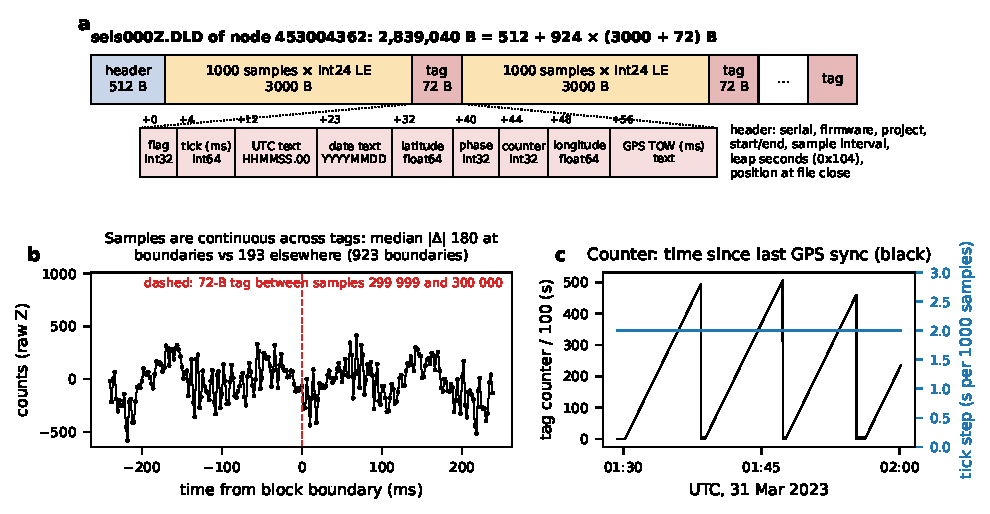
\includegraphics[width=\textwidth]{figures/fig02_dld_format.pdf}
\caption{The DLD format. (a) File layout and the 72-byte tag after every 1000 samples (byte offsets within the tag). (b) Raw samples around a block boundary of node 453004362: the tag interrupts the byte stream but not the signal; the median absolute sample-to-sample difference at the 923 boundaries equals that elsewhere. (c) Tag counter (time since the last GPS synchronisation) and tick step (2~s per 1000 samples, i.e.\ 500~sps).}
\label{fig:dld}
\end{figure*}

\paragraph{Timing.} The time text in each tag looks like the obvious time stamp, but it is not reliable at the 2-s level. In files whose header leap-second field is 0, the text time is exactly 2~s later than the time derived from the TOW. In files whose field is 18, the two agree. Files that span the moment the receiver learns the current GPS--UTC offset show the text time jumping back by 2~s in mid-file, for example a repeated \code{00:58:37} after block 2197 in one of our files. We interpret this as the receiver using an outdated default offset of 16~s until the almanac delivers the current value of 18~s. The TOW is continuous across such jumps. As in common GPS timing receivers, it is the time of the next pulse per second. node\_toolbox therefore computes the UTC time of a tag as
\begin{equation}\label{eq:tow}
t_\mathrm{UTC} = t_0 + 604800\,W + \frac{\mathrm{TOW}}{1000} - 1 - \Delta t_\mathrm{LS},
\end{equation}
where $t_0$ is the GPS epoch (1980-01-06), $W$ the GPS week (from the tag date), TOW in ms, and $\Delta t_\mathrm{LS}$ the GPS--UTC leap-second offset at that time (18~s since 2017). This is the default (\code{time\_source="tow"}). The text time remains available, and the difference between the two is reported for every tag (\code{label\_minus\_tow\_s}). Section~\ref{sec:timing} shows the effect between nodes.

One convention remains unverified: whether a tag time refers to the first sample of the block before it (default, \code{tag\_marks="block\_start"}) or to the sample after the block. The alternative shifts all samples by one block (1, 2 or 4~s). Because the time of the first sample cannot be cross-checked between nodes, this needs one comparison with a SoloLite export of the same file. \code{compare\_with\_export} does this comparison.

\code{read\_dld} returns an ObsPy \code{Stream} for any time window, reading only the blocks needed. Gaps (a change of tick step or a time jump) start a new trace. The function \code{read\_dld\_node} reads the three components of a power-up, \code{scan\_dld} lists the continuous segments without reading samples, and \code{convert\_dld} converts a whole drive. Files are opened read-only and are never modified, which a unit test confirms.

\subsection{Waveforms, codes and metadata}

\code{index\_waveforms} builds a table of all waveform files under a directory, including \code{.DLD}, MiniSEED and SEG-Y, with serial, component, start and end. It can cache the table as CSV. \code{extract\_waveforms} cuts the selected window for each selected deployment, merges and trims it, assigns SEED codes \citep{fdsn_seed_2012} and writes MiniSEED or SEG-Y files with one file per channel and window. Window ends are exclusive, so consecutive windows do not share samples.

\paragraph{Codes.} Network, station and location codes come from an optional mapping table (serial to codes, optionally with validity times). Without a row, the station code defaults to the last five digits of the serial. The band code follows the sample rate (\code{D} at 250 and 500~sps, \code{G} at 1000~sps), the instrument code is \code{P} (short-period geophone), and the node axes X and Y map to N and E \citep{dtcc_manual}, giving, e.g., \code{DPZ}, \code{DPN}, \code{DPE}.

\paragraph{Polarity.} The SmartSolo manual defines positive output for case motion to the south, west and down \citep{dtcc_manual}. Controlled tests by AusPass confirm negative polarity for all three IGU-16HR channels relative to FDSN convention \citep{auspass_data}. \code{extract\_waveforms} therefore multiplies IGU-16HR data by $-1$ by default (\code{invert\_polarity="auto"}). It records this in the trace header (\code{stats.processing}), and \code{build\_inventory} writes the channel orientation to match.

\paragraph{Gain and response.} Raw DLD counts include the preamplifier gain $G$ (in dB, from the log). The AusPass response for gain-removed data has zeros at 0 (twice), poles at $p_{1,2} = -22.211059 \pm 22.217768\,i$~rad/s (5~Hz, damping 0.707) and a flat high-frequency sensitivity of $257\,019\,225.55$~counts/(m/s) \citep{auspass_nodes}. \code{build\_inventory(response="auspass")} writes
\begin{equation}\label{eq:resp}
H(s) = S_0\,10^{G/20}\,\frac{s^2}{(s-p_1)(s-p_2)},
\end{equation}
with $S_0$ the AusPass sensitivity and $G$ taken from each deployment (\code{gain\_db="auto"}), or 0 for exports with the gain already removed. Alternatives are a nominal response from the boot-test values or no response. Positions, elevations, sample rate, azimuth and dip complete each channel. StationXML is written through ObsPy.

\subsection{Sensor quality control and orientation}

\paragraph{Boot-time geophone test.} At every power-up the node measures coil resistance, natural frequency $f_0$, damping $h$, sensitivity and noise for each channel and logs a pass flag. \code{smartsolo\_node.geophone\_qc} compares the values with the limits in the node's own script (\code{sct\_par.xml}). It also flags tests whose spread noise exceeds a threshold (default 5000). A test taken while the node is being moved can be logged as passed although its damping and sensitivity are out of specification.

\paragraph{Pulse test.} \code{PULSE\_\{X,Y,Z\}.WAV} contains 16\,000 samples of 24-bit data whose header claims 10~kHz. The content is a 16-s sequence of current steps followed by a quiet section. This matches the geophone/ADC test stage described in the manual \citep{dtcc_manual} at a fixed rate of 1000~sps, independent of the acquisition rate. \code{analyse\_pulse} finds the steps and fits a damped oscillation
\begin{equation}\label{eq:pulse}
x(t) = A\, e^{-h\omega_0 t} \sin\!\left(\omega_0\sqrt{1-h^2}\,t + \phi\right) + C,\qquad \omega_0 = 2\pi f_0,
\end{equation}
to the 0.9~s after each switch-off. It measures the noise floor in the quiet section and converts counts to volts with 3355.4428~counts/mV at 0~dB \citep{dtcc_manual}.

\paragraph{Orientation.} The eCompass heading, tilt, roll and pitch are logged regularly. \code{smartsolo\_orientation} provides circular statistics and separates boot-time readings, taken before the node is planted, from the settled heading. It measures rotation over a deployment and computes the IGRF-13 \citep{alken_igrf13_2021} declination and field at each site. It can write azimuths to StationXML or rotate data to north and east. Because it is not documented whether \code{eCompass North} is a magnetic azimuth of the node's arrow, nor whether the compass was calibrated, the package reports both the raw heading and the heading corrected for declination, and leaves the choice to the user.

%-----------------------------------------
\section{Verification and test cases}

The repository includes 14 unit tests (\code{pytest}). They cover:
\begin{itemize}
\item record counts against log headers for all bundled logs and a V1.1.4 GNSS log;
\item deployment splitting for a synthetic node that was moved;
\item radius, polygon and time selection;
\item DLD block decoding, sample-rate detection and continuity across tags;
\item the 2-s label offset;
\item alignment of neighbouring nodes;
\item the read-only guarantee;
\item a round trip from DLD to MiniSEED and SEG-Y that checks the exported data are exactly $-1$ times the raw counts.
\end{itemize}
Five Jupyter notebooks reproduce the examples below and serve as tutorials.

\subsection{State of health on the Antarctic ice}

Two nodes (453021267 and 453022522, firmware V1.0.8.1be, 1000~sps, 0~dB) were deployed at 1644--1649~m elevation in Dronning Maud Land, Antarctica (71.55$^\circ$S, 11.12$^\circ$E) from 25 December 2024 to 8 January 2025. Their logs (2.1~MB each, about 9900 records) also contain bench and transport boots from November 2024. The parser separates these into their own sessions. Figure~\ref{fig:soh} shows four of the logged quantities against time.
\begin{itemize}
\item \textbf{Temperature} follows a daily cycle between $-17.4$ and $+7.7^\circ$C.
\item \textbf{Battery voltage} falls from 8.25 to 7.63~V over 13.8 days at 1000~sps.
\item \textbf{Tilt} is constant at 1.7$^\circ$ and 5.1$^\circ$; the second node exceeds the 3$^\circ$ specification for the horizontal geophones.
\item \textbf{Heading} is stable to 0.9$^\circ$ (circular standard deviation). Node 453021267 nevertheless rotates by 2.3$^\circ$ over the deployment (0.17$^\circ$/day) at constant tilt, which points to ice motion or compass drift.
\end{itemize}
The IGRF declination at the site is $-29.5^\circ$ (inclination $-61.3^\circ$, horizontal field 19\,000~nT).

\begin{figure*}[ht!]
\centering
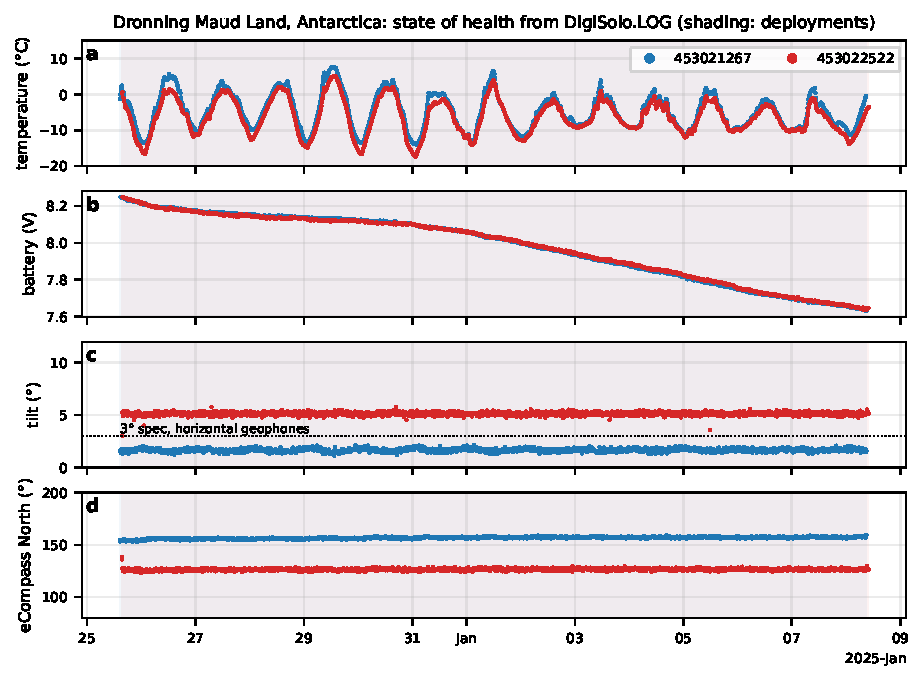
\includegraphics[width=\textwidth]{figures/fig03_state_of_health.pdf}
\caption{State of health of two nodes in Dronning Maud Land read with \code{read\_logs}: (a) temperature, (b) battery voltage, (c) tilt with the 3$^\circ$ horizontal-geophone specification, (d) eCompass heading. Shading marks the deployments found by \code{build\_deployments}.}
\label{fig:soh}
\end{figure*}

The first-stable-fix rule matters in practice (Fig.~\ref{fig:loc}). For 453022522 the first two fixes after the cold start were 45--100~m from the final position and are skipped. All later fixes scatter by a few metres. The median position moves by 2.6 and 3.1~m over two weeks, about 0.2~m/day, which is within GPS noise but consistent with ice flow.

\begin{figure*}[ht!]
\centering
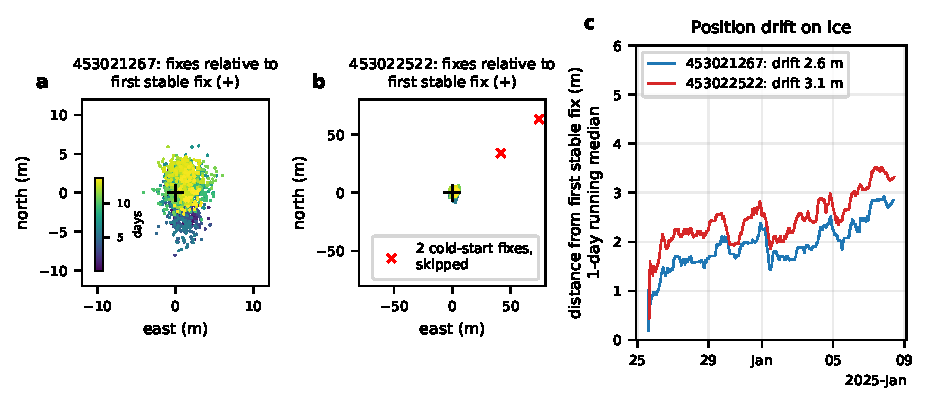
\includegraphics[width=\textwidth]{figures/fig04_location.pdf}
\caption{GPS positions in the logs of the two Antarctic nodes relative to the first stable fix (a, b; colour: days after power-up; crosses: cold-start fixes that are skipped) and 1-day running median distance from the first stable fix (c).}
\label{fig:loc}
\end{figure*}

\subsection{Pulse test and boot-time test}

Figure~\ref{fig:pulse} shows the pulse file of 453022522 and the fit of Eq.~\ref{eq:pulse} after a switch-off. Across 21 channels of seven nodes (one Antarctic node and the six nodes of the braking test), the fitted $f_0$ and $h$ agree with the values the node logged at the same boot, with median absolute differences of 0.06~Hz and 0.011. The noise floor of the quiet section is 1.13--1.26~$\mu$V, equal to the logged RMS noise. This confirms both the 1000-sps rate of the pulse file and the counts-per-volt conversion. The pulse file of the braking-test nodes, which recorded at 500~sps, is also at 1000~sps.

The boot-time test also exposed handling problems:
\begin{itemize}
\item One Antarctic node and one braking-test node tested themselves while being carried (spread noise up to 22\,000 and 144\,000). Both logged a pass although their damping and sensitivity were out of limits.
\item Another node returned an implausible $f_0$ of 78~kHz on one channel without being noisy, but tested normally at its next boot.
\item Coil resistance follows temperature as expected for copper: about 1620~$\Omega$ at $-2^\circ$C and 1730--1780~$\Omega$ at room temperature.
\end{itemize}

\begin{figure*}[ht!]
\centering
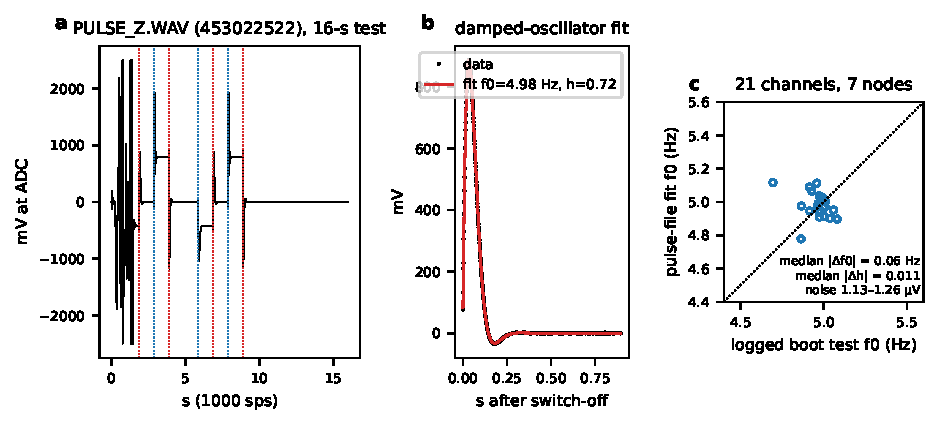
\includegraphics[width=\textwidth]{figures/fig05_pulse_test.pdf}
\caption{Pulse test. (a) \code{PULSE\_Z.WAV} of node 453022522 read at 1000~sps (dotted lines: detected current steps). (b) Damped-oscillator fit (Eq.~\ref{eq:pulse}) after a switch-off. (c) Natural frequency from the pulse file against the value logged by the node at the same boot, 21 channels of seven nodes.}
\label{fig:pulse}
\end{figure*}

\subsection{Timing between nodes}\label{sec:timing}

The 2-s label offset is easy to miss because nodes deployed together usually share it. In all six braking-test files the header leap-second field is 0 and the text time is exactly 2~s ahead of Eq.~\ref{eq:tow} in every tag (Fig.~\ref{fig:timing}c). Relative timing between those nodes is therefore unaffected.

Problems appear when nodes in one dataset differ. In a longer recording of four of the same nodes (not included in the repository), the text times jumped back by 2~s at different times on different nodes (23:56, 00:21, 00:58 and 02:38~UTC). Cross-correlating ambient noise between node pairs every 10~minutes gave lags of exactly $\pm2$~s whenever one node's text time had jumped and the other's had not. With TOW times the lags were $0\pm4$~ms throughout. We saw the same 2-s offset in files from firmware V1.1.2 at 250~sps. Two of those nodes, 10~m apart, started 4~s apart, yet their records aligned to within one sample at a correlation of 0.96. This confirms the block decoding and the TOW timing independently of the braking test.

Within the braking test, neighbouring nodes 5 and 12~m apart give median lags of $-6$ and $+30$~ms in 30-s windows (Fig.~\ref{fig:timing}b). The scatter of individual windows reflects the moving vehicle sources rather than timing.

\begin{figure*}[ht!]
\centering
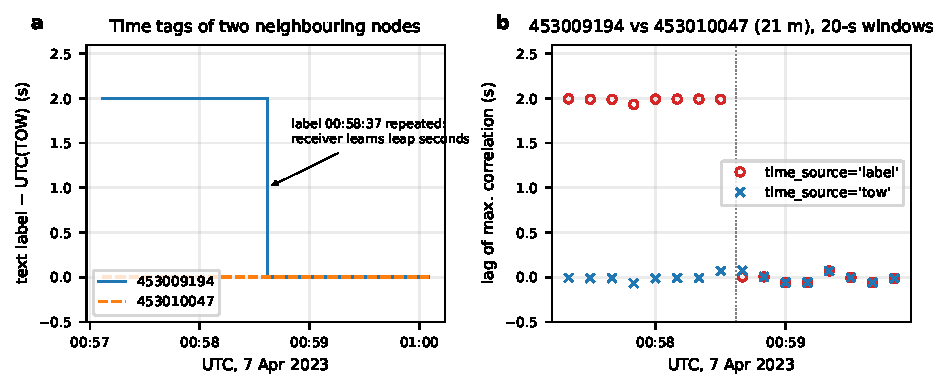
\includegraphics[width=\textwidth]{figures/fig06_timing.pdf}
\caption{Timing. (a) Schematic: the text time in each tag is 2~s late until the GPS receiver knows the current leap seconds, while the GPS time of week (TOW, Eq.~\ref{eq:tow}) is not affected. (b) Lag of maximum cross-correlation between neighbouring nodes using TOW times. (c) Text time minus TOW-derived UTC and the header leap-second field for all six braking-test files.}
\label{fig:timing}
\end{figure*}

\subsection{A six-node braking test}

The end-to-end example uses six complete nodes (firmware V1.0.5.6kp, 500~sps, 0~dB) that recorded for about 30~minutes on 31 March 2023 (01:28--02:00~UTC) along a road beside the sports oval in Sandy Bay, Hobart, Tasmania. The source was a Toyota Land Cruiser HJ60 braking repeatedly, about ten times; the exact times were not noted. A laughing baby rode in the back seat but was not detected. The nodes formed a group of three in the south-west (453004362, 453009194 and 453010047, 5--21~m apart), one node 41~m to the north-east (453010029) and a pair (453010077 and 453010167, 12~m apart) about 110~m from the first group (Fig.~\ref{fig:map}). The raw DLD files of all nodes are included in the repository (about 45~MB, Git LFS).

Positions from the DLD tags place the nodes and show that five of them were carried 70--230~m while still recording after 01:51. A 30-m radius around the north-east pair and a polygon around the south-west group select the expected nodes (Fig.~\ref{fig:map}; Listing~\ref{code:select}).

\begin{figure}[ht!]
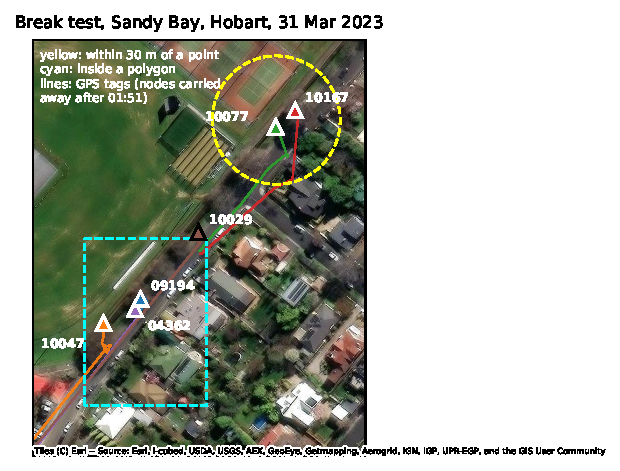
\includegraphics[width=8.6cm]{figures/fig07_selection_map.pdf}
\caption{Braking-test nodes on 31 March 2023 positioned from the DLD tags, with tag tracks showing the nodes being carried away at the end. Dashed: a 30-m radius selection (yellow) and a polygon selection (cyan); selected nodes have white outlines. Imagery: Esri World Imagery via contextily \citep{contextily}.}
\label{fig:map}
\end{figure}

Figure~\ref{fig:break} shows results from the raw files.
\begin{itemize}
\item \textbf{Envelopes} show regular vehicle passes between 01:34 and 01:50 and the much stronger signals of handling afterwards (Fig.~\ref{fig:break}a).
\item \textbf{Exported record section.} The Z channels exported as MiniSEED (codes \code{??.DPZ}, polarity inverted) show the passing vehicle node by node (Fig.~\ref{fig:break}b). The spectrogram has a broadband burst at closest approach and gliding tonal lines from the engine and drivetrain (Fig.~\ref{fig:break}c).
\item \textbf{Events and speeds.} Peaks of the envelope at least eight times the background, seen by both nodes of a pair within 5~s, give 9 and 24 events at the two pairs. Matching events between the pairs gives 14 passes with a median apparent speed of 41~km/h (Fig.~\ref{fig:break}d). This is consistent with a car slowing, stopping and pulling away.
\item \textbf{Spectra.} The events raise the spectrum by two to three orders of magnitude between 5 and 100~Hz (Fig.~\ref{fig:break}e).
\end{itemize}
The exported MiniSEED and SEG-Y samples equal $-1$ times the raw DLD counts exactly, and their start times equal the TOW-derived DLD times.

\begin{figure*}[ht!]
\centering
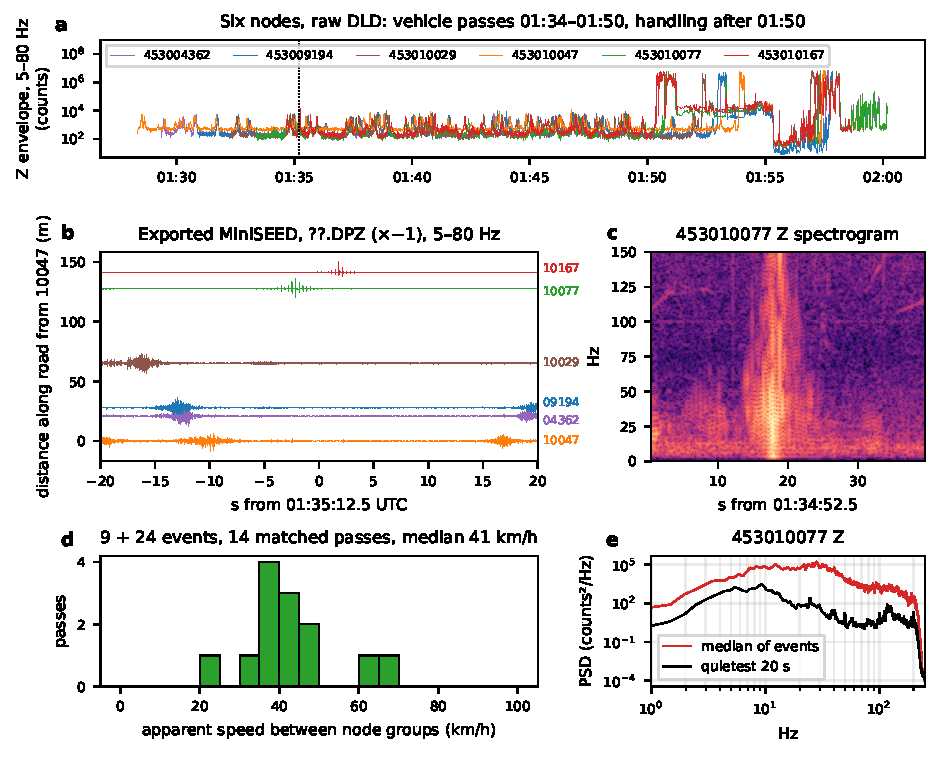
\includegraphics[width=\textwidth]{figures/fig08_break_test.pdf}
\caption{Braking test. (a) Vertical-component envelopes (5--80~Hz) of all six nodes read from the raw DLD files; dotted line: the event in (b, c). (b) Record section of the exported MiniSEED (polarity corrected), ordered by distance along the road. (c) Spectrogram of 453010077. (d) Apparent speeds from the travel time between the two node groups. (e) Median spectrum of the events and the quietest 20~s at 453010077.}
\label{fig:break}
\end{figure*}

%-----------------------------------------
\section{Performance}

Table~\ref{tab:perf} lists execution times on a two-core 2.9-GHz Intel Xeon virtual machine (Python 3.14, ObsPy 1.5.1, pandas 3.0). Reading a 31-minute, 500-sps DLD component (2.8~MB) takes 77~ms, about 24\,000 times faster than real time. A 60-s window takes about the same, because the time tags of the whole file are decoded first. One day of continuous 1000-sps data is about 265~MB per component in DLD and is read in about 7~s at the same rate. Log parsing is the slowest step, at about 1.7~s per two-week log with 9900 records. It runs once per node, and the deployment and waveform index tables can be cached as CSV.

\begin{table}[ht!]
\seismicatablestyle
\begin{tabular}{m{4.9cm} m{2.4cm}}
Operation & Time \\
\hline
DLD header & 0.06 ms \\
DLD time tags (924 blocks) & 36 ms \\
DLD full component (924\,000 samples) & 77 ms \\
DLD 60-s window & 66 ms \\
Log, 2.1~MB, 9920 records & 1.7 s \\
Deployments from two logs & 3.5 s \\
Deployments from 18 DLD files & 0.58 s \\
Waveform index, 18 DLD files & 1.1 s \\
\end{tabular}
\caption{Median execution times (5 repetitions; 3 for the last four rows).}
\label{tab:perf}
\end{table}

%-----------------------------------------
\section{Limitations}

The DLD description is derived from files of four firmware versions. Other versions may differ; \code{read\_dld} checks the magic string and the presence and spacing of the time tags, and raises an error if they are not as expected. Three conventions remain to be confirmed:
\begin{itemize}
\item the block convention of the time tags;
\item the mapping of the logged channels 1--3 to the X, Y and Z axes;
\item the meaning of \code{eCompass North}.
\end{itemize}
The first needs one comparison with a SoloLite export, which the package supports, and the others need controlled orientation tests. We have not handled the BD3C-5 broadband variant, for which AusPass reports no polarity inversion \citep{auspass_data}; it is excluded from the automatic polarity flip by its device type. The pulse-test model (Eq.~\ref{eq:pulse}) is fitted to the switch-off after a negative current. After a positive current it gives about 5.35~Hz, which suggests a non-linear suspension at larger drive.

%-----------------------------------------
\section{Conclusions}

node\_toolbox reads all files written by SmartSolo IGU-16HR nodes with open-source Python and connects them to standard seismological formats and tools. It makes three practical points explicit that are easy to get wrong:
\begin{itemize}
\item The logged sample rate is a sample interval.
\item The time text in raw data tags is 2~s late until the receiver knows the leap seconds, whereas the GPS time of week is reliable.
\item IGU-16HR data need a polarity inversion, and raw counts include the preamplifier gain.
\end{itemize}
The deployment logic keeps each power-up separate and places it at the first stable GPS position, which protects against cold-start errors and moved nodes. The state-of-health and quality-control tools turn the logs, which are rarely used, into information for field crews and station metadata. The code, tests, example data and tutorials are openly available, and we welcome contributions of files from other firmware versions.

\begin{acknowledgements}
We thank AusPass for publishing their SmartSolo polarity and response tests. Part of the code and text was drafted with the assistance of an AI tool (Perplexity Computer) and checked by the author. % TODO: funding, field support, co-authors; check the journal's AI-disclosure policy
\end{acknowledgements}

\section*{Data and code availability}
The code, unit tests, tutorial notebooks, figure scripts (\code{paper/make\_figures.py}) and example data are available at \url{https://github.com/TobbeTripitaka/node_toolbox} under the MIT licence \citep{node_toolbox}. A versioned snapshot will be archived on Zenodo upon acceptance (DOI to be added). The repository contains the state-of-health logs and pulse-test files of the two Antarctic nodes and the complete files, including raw DLD data, of the six braking-test nodes (Git LFS). The user manual consists of the repository README, the module docstrings, \code{docs/DLD\_FORMAT.md}, \code{docs/FINDINGS.md} and the notebooks. Basemap imagery in Fig.~\ref{fig:map} is Esri World Imagery (sources: Esri, i-cubed, USDA, USGS, AEX, GeoEye, Getmapping, Aerogrid, IGN, IGP, UPR-EGP and the GIS User Community).

\section*{Competing interests}
The authors have no competing interests. node\_toolbox is independent of, and not endorsed by, DTCC or SmartSolo.

\bibliography{references}

\end{document}
